\documentclass[11pt]{article}
\usepackage[letterpaper,margin=.7in]{geometry}
\usepackage[T1]{fontenc}
\usepackage{lmodern}
\usepackage{amsmath,amssymb}
\usepackage[dvipsnames]{xcolor}
\usepackage{tikz}
\usetikzlibrary{arrows.meta,calc,decorations.markings,positioning}
\usepackage{caption}
\captionsetup{font=small,labelfont=bf}
\definecolor{TYordinary}{HTML}{1F5F7A}
\definecolor{TYcharacter}{HTML}{A33A2B}
\definecolor{TYprojector}{HTML}{167C78}
\definecolor{TYauxiliary}{HTML}{6B7280}

\tikzset{
  kirby component/.style={line width=1.05pt,line cap=round,line join=round},
  ordinary component/.style={kirby component,draw=TYordinary},
  ribbon strand/.style={line width=1.1pt,draw=TYordinary,-{Stealth[length=4pt]}},
  plain strand/.style={line width=1.1pt,draw=TYordinary},
  character coupon/.style={draw=TYcharacter,fill=white,line width=.8pt,
    minimum width=8mm,minimum height=4.5mm,font=\scriptsize,text=TYcharacter},
  projector coupon/.style={draw=TYprojector,fill=TYprojector!7,line width=.9pt,
    minimum width=12mm,minimum height=6mm,font=\scriptsize,text=TYprojector},
  fusion vertex/.style={circle,fill=black,inner sep=1.35pt},
  boundary point/.style={circle,fill=black,inner sep=1.7pt},
  flow arrow/.style={-{Stealth[length=5pt]},line width=.8pt,draw=black!65},
  context box/.style={draw=black!45,dashed,rounded corners=2pt,line width=.7pt},
  panel label/.style={font=\small\bfseries,anchor=north west},
  semantic label/.style={font=\footnotesize,align=center,text=black!75}
}


\title{Candidate Diagram Gallery}
\author{Homologically Twisted Crane--Yetter Invariants}
\date{Draft for mathematical review}

\begin{document}
\maketitle

These diagrams are candidates, not yet normative figures.  Each caption
states the sole mathematical role intended for the corresponding picture.

\begin{figure}[ht]
  \centering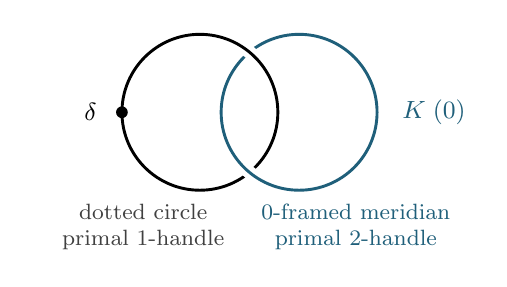
\begin{tikzpicture}[scale=.9]
  \draw[kirby component] (-0.7,0) circle[radius=1.1];
  \draw[ordinary component,preaction={draw=white,line width=4.8pt}]
    (0.7,0) circle[radius=1.1];
  \draw[kirby component,preaction={draw=white,line width=4.8pt}]
    (-0.7,0) ++(43:1.1) arc[start angle=43,end angle=59,radius=1.1];
  \fill (-1.8,0) circle[radius=2.35pt];
  \node[font=\small,anchor=east] at (-2.02,0) {$\delta$};
  \node[font=\small,text=TYordinary,anchor=west] at (2.02,0) {$K\;(0)$};
  \node[semantic label,text width=2.7cm] at (-1.5,-1.62)
    {dotted circle\\primal $1$-handle};
  \node[semantic label,text=TYordinary,text width=2.9cm] at (1.5,-1.62)
    {$0$-framed meridian\\primal $2$-handle};
\end{tikzpicture}

  \caption{Kirby notation tested on the standard canceling $1$--$2$ pair.}
\end{figure}

\begin{figure}[ht]
  \centering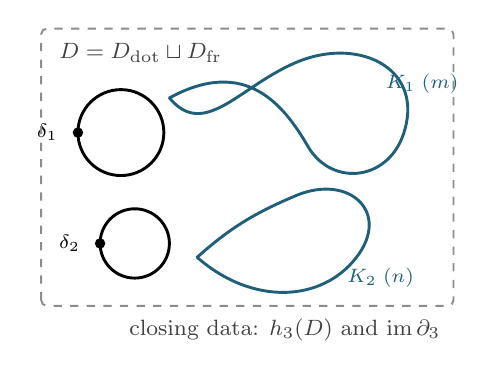
\begin{tikzpicture}[scale=.88]
  % A schematic closed framed link: no manifold is assigned to this picture.
  \draw[kirby component] (-2.25,.75) circle[radius=.62];
  \fill (-2.87,.75) circle[radius=2.15pt];
  \node[font=\scriptsize,anchor=east] at (-3.02,.75) {$\delta_1$};
  \draw[kirby component] (-2.05,-.85) circle[radius=.5];
  \fill (-2.55,-.85) circle[radius=2.15pt];
  \node[font=\scriptsize,anchor=east] at (-2.7,-.85) {$\delta_2$};

  \draw[ordinary component]
    (-1.55,1.25)
      .. controls (-.45,1.85) and (.1,1.15) .. (.45,.55)
      .. controls (.8,-.05) and (1.65,.05) .. (1.85,.8)
      .. controls (2.1,1.7) and (1.15,2.15) .. (.25,1.75)
      .. controls (-.55,1.4) and (-1.05,.65) .. (-1.55,1.25);
  \node[font=\scriptsize,text=TYordinary] at (2.1,1.45) {$K_1\;(m)$};

  \draw[ordinary component]
    (-1.15,-1.05)
      .. controls (-.35,-1.75) and (.65,-1.7) .. (1.15,-1.05)
      .. controls (1.65,-.4) and (1.05,.15) .. (.3,-.15)
      .. controls (-.35,-.42) and (-.7,-.65) .. (-1.15,-1.05);
  \node[font=\scriptsize,text=TYordinary] at (1.5,-1.35) {$K_2\;(n)$};

  \draw[context box] (-3.4,-1.75) rectangle (2.55,2.25);
  \node[semantic label,anchor=north west] at (-3.28,2.18)
    {$D=D_{\mathrm{dot}}\sqcup D_{\mathrm{fr}}$};
  \node[semantic label,anchor=north east] at (2.5,-1.8)
    {closing data: $h_3(D)$ and $\operatorname{im}\partial_3$};
\end{tikzpicture}

  \caption{Schematic anatomy of a special Kirby representative.  No
  four-manifold is assigned to this particular link.}
\end{figure}

\clearpage
\begin{figure}[ht]
  \centering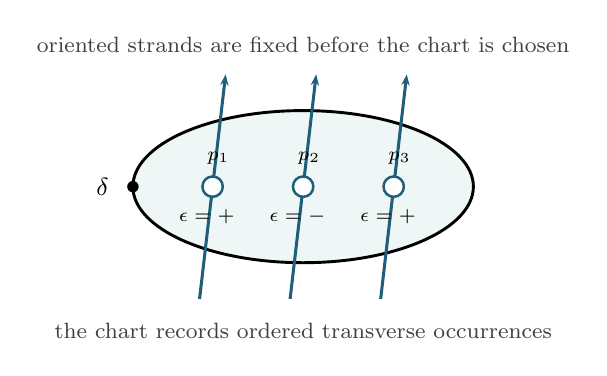
\begin{tikzpicture}[scale=.92]
  \fill[TYprojector!7] (0,0) ellipse[x radius=2.35,y radius=1.05];
  \draw[kirby component] (0,0) ellipse[x radius=2.35,y radius=1.05];
  \fill (-2.35,0) circle[radius=2.25pt];
  \node[font=\small,anchor=east] at (-2.55,0) {$\delta$};

  \foreach \x/\lab/\sgn in {-1.25/p_1/+,0/p_2/-,1.25/p_3/+} {
    \draw[ribbon strand] (\x-.18,-1.55) -- (\x+.18,1.55);
    \fill[white] (\x,0) circle[radius=4pt];
    \draw[TYordinary,line width=.9pt] (\x,0) circle[radius=4pt];
    \node[font=\scriptsize,anchor=south] at (\x+.08,.18) {$\lab$};
    \node[font=\scriptsize,anchor=north] at (\x-.08,-.18) {$\epsilon=\sgn$};
  }
  \node[semantic label,anchor=south] at (0,1.72)
    {oriented strands are fixed before the chart is chosen};
  \node[semantic label,anchor=north] at (0,-1.75)
    {the chart records ordered transverse occurrences};
\end{tikzpicture}

  \caption{A dotted co-core chart records finitely many ordered transverse
  strand occurrences.  It does not choose the labels $X$ versus $X^*$.}
\end{figure}

\begin{figure}[ht]
  \centering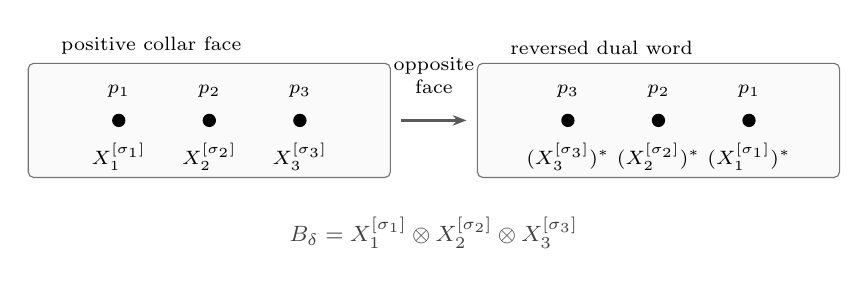
\begin{tikzpicture}[scale=.92]
  \node[draw=black!55,rounded corners=2pt,minimum width=4.6cm,
    minimum height=1.45cm,fill=black!2] (plus) at (-3.1,0) {};
  \node[font=\scriptsize,anchor=south west] at (-5.28,.78)
    {positive collar face};
  \foreach \x/\j/\obj in {-4.35/1/X_1^{[\sigma_1]},-3.1/2/X_2^{[\sigma_2]},-1.85/3/X_3^{[\sigma_3]}} {
    \node[boundary point] at (\x,0) {};
    \node[font=\scriptsize,anchor=south] at (\x,.18) {$p_\j$};
    \node[font=\scriptsize,anchor=north] at (\x,-.18) {$\obj$};
  }

  \draw[flow arrow] (-.45,0) -- (.45,0);
  \node[font=\scriptsize,align=center] at (0,.62) {opposite\\face};

  \node[draw=black!55,rounded corners=2pt,minimum width=4.6cm,
    minimum height=1.45cm,fill=black!2] (minus) at (3.1,0) {};
  \node[font=\scriptsize,anchor=south west] at (.92,.78)
    {reversed dual word};
  \foreach \x/\j/\obj in {1.85/3/(X_3^{[\sigma_3]})^*,3.1/2/(X_2^{[\sigma_2]})^*,4.35/1/(X_1^{[\sigma_1]})^*} {
    \node[boundary point] at (\x,0) {};
    \node[font=\scriptsize,anchor=south] at (\x,.18) {$p_\j$};
    \node[font=\scriptsize,anchor=north] at (\x,-.18) {$\obj$};
  }
  \node[semantic label] at (0,-1.55)
    {$B_\delta=X_1^{[\sigma_1]}\otimes X_2^{[\sigma_2]}\otimes X_3^{[\sigma_3]}$};
\end{tikzpicture}

  \caption{The two faces of a cut-open dotted handle carry mutually reversed
  dual boundary words.}
\end{figure}

\clearpage
\begin{figure}[ht]
  \centering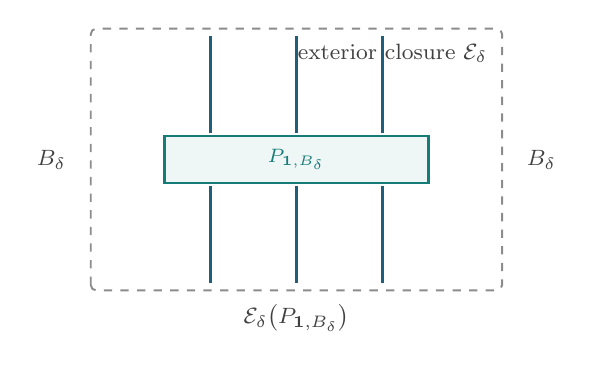
\begin{tikzpicture}[scale=.95]
  \draw[context box] (-2.75,-1.75) rectangle (2.75,1.75);
  \node[semantic label,anchor=north east] at (2.68,1.68)
    {exterior closure $\mathcal E_\delta$};
  \foreach \x in {-1.15,0,1.15} {
    \draw[plain strand] (\x,-1.65) -- (\x,-.35);
    \draw[plain strand] (\x,.35) -- (\x,1.65);
  }
  \node[projector coupon,minimum width=3.35cm] at (0,0)
    {$P_{\mathbf1,B_\delta}$};
  \node[semantic label] at (0,-2.12)
    {$\mathcal E_\delta\!\left(P_{\mathbf1,B_\delta}\right)$};
  \node[semantic label,anchor=east] at (-2.95,0)
    {$B_\delta$};
  \node[semantic label,anchor=west] at (2.95,0)
    {$B_\delta$};
\end{tikzpicture}

  \caption{The dotted operation is the tensor-unit projector inserted into
  the actual exterior closure context.}
\end{figure}

\begin{figure}[ht]
  \centering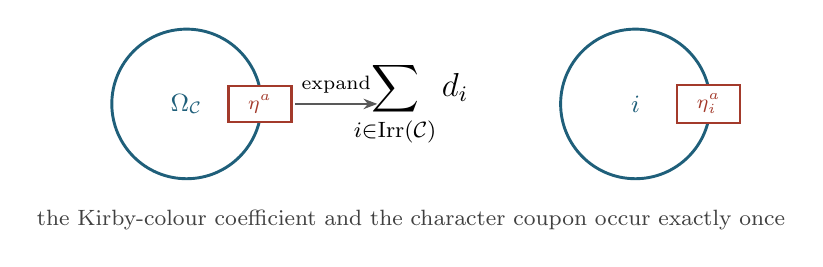
\begin{tikzpicture}[scale=.95]
  \draw[ordinary component] (-3,0) circle[radius=1];
  \node[font=\small,text=TYordinary] at (-3,0) {$\Omega_{\mathcal C}$};
  \node[character coupon] at (-2.02,0) {$\eta^a$};

  \draw[flow arrow] (-1.55,0) -- (-.45,0)
    node[midway,above,font=\scriptsize] {expand};
  \node[font=\large] at (0,0) {$\displaystyle\sum_{i\in\operatorname{Irr}(\mathcal C)}d_i$};

  \draw[ordinary component] (3,0) circle[radius=1];
  \node[font=\small,text=TYordinary] at (3,0) {$i$};
  \node[character coupon] at (3.98,0) {$\eta_i^a$};
  \node[semantic label] at (0,-1.55)
    {the Kirby-colour coefficient and the character coupon occur exactly once};
\end{tikzpicture}

  \caption{An ordinary component is expanded in the Kirby colour and carries
  its homological character coupon.}
\end{figure}

\clearpage
\begin{figure}[ht]
  \centering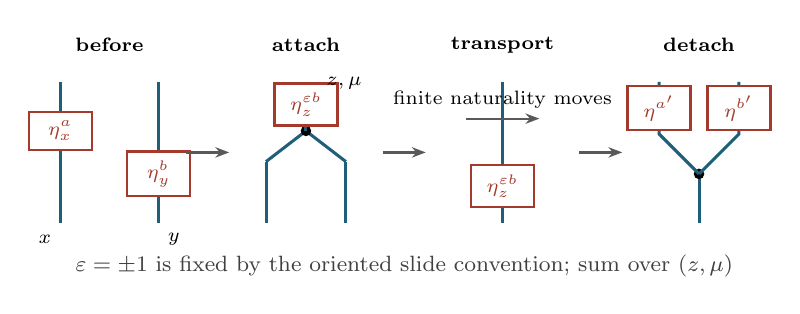
\begin{tikzpicture}[scale=.78]
  \foreach \shift/\title in {0/before,3.2/attach,6.4/transport,9.6/detach} {
    \node[font=\scriptsize\bfseries] at (\shift,1.75) {\title};
  }

  % before
  \draw[plain strand] (-.8,-1.15) -- (-.8,1.15);
  \draw[plain strand] (.8,-1.15) -- (.8,1.15);
  \node[font=\scriptsize] at (-1.05,-1.42) {$x$};
  \node[font=\scriptsize] at (1.05,-1.42) {$y$};
  \node[character coupon] at (-.8,.35) {$\eta_x^a$};
  \node[character coupon] at (.8,-.35) {$\eta_y^b$};

  % attach to an internal channel z
  \draw[plain strand] (2.55,-1.15) -- (2.55,-.15);
  \draw[plain strand] (3.85,-1.15) -- (3.85,-.15);
  \draw[plain strand] (2.55,-.15) -- (3.2,.35);
  \draw[plain strand] (3.85,-.15) -- (3.2,.35);
  \node[fusion vertex] at (3.2,.35) {};
  \draw[plain strand] (3.2,.35) -- (3.2,1.15);
  \node[character coupon] at (3.2,.78) {$\eta_z^{\varepsilon b}$};
  \node[font=\scriptsize] at (3.82,1.12) {$z,\mu$};

  % transport along the internal channel
  \draw[plain strand] (6.4,-1.15) -- (6.4,1.15);
  \node[character coupon] at (6.4,-.55) {$\eta_z^{\varepsilon b}$};
  \draw[flow arrow] (5.8,.55) -- (7,.55)
    node[midway,above,font=\scriptsize] {finite naturality moves};

  % detach
  \draw[plain strand] (9.6,-1.15) -- (9.6,-.35);
  \node[fusion vertex] at (9.6,-.35) {};
  \draw[plain strand] (9.6,-.35) -- (8.95,.3) -- (8.95,1.15);
  \draw[plain strand] (9.6,-.35) -- (10.25,.3) -- (10.25,1.15);
  \node[character coupon] at (8.95,.72) {$\eta^{a'}$};
  \node[character coupon] at (10.25,.72) {$\eta^{b'}$};

  \foreach \x in {1.6,4.8,8.0} {
    \draw[flow arrow] (\x-.35,0) -- (\x+.35,0);
  }
  \node[semantic label] at (4.8,-1.85)
    {$\varepsilon=\pm1$ is fixed by the oriented slide convention; sum over $(z,\mu)$};
\end{tikzpicture}

  \caption{Proof architecture for an oriented $2/2$ slide: attach, finite
  coupon transport, and detach.  The exact sign convention remains visible.}
\end{figure}

\begin{figure}[ht]
  \centering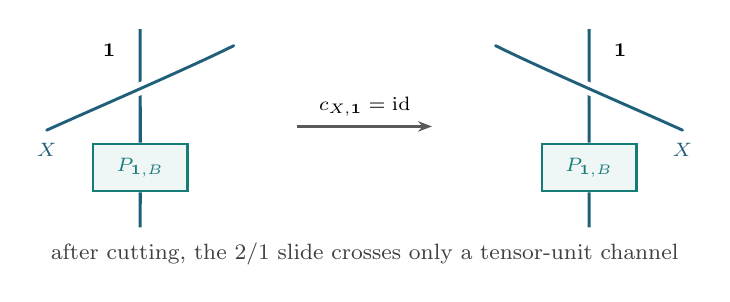
\begin{tikzpicture}[scale=.95]
  \node[projector coupon] (p1) at (-3,-.55) {$P_{\mathbf1,B}$};
  \draw[plain strand] (-3,-1.35) -- (p1.south);
  \draw[plain strand] (p1.north) -- (-3,1.3);
  \node[font=\scriptsize,anchor=east] at (-3.2,1.02) {$\mathbf1$};
  \draw[ordinary component,preaction={draw=white,line width=4.5pt}]
    (-4.25,-.05) .. controls (-3.7,.2) and (-2.35,.78) .. (-1.75,1.08);
  \node[font=\scriptsize,text=TYordinary] at (-4.25,-.32) {$X$};

  \draw[flow arrow] (-.9,0) -- (.9,0)
    node[midway,above,font=\scriptsize] {$c_{X,\mathbf1}=\operatorname{id}$};

  \node[projector coupon] (p2) at (3,-.55) {$P_{\mathbf1,B}$};
  \draw[plain strand] (3,-1.35) -- (p2.south);
  \draw[plain strand] (p2.north) -- (3,1.3);
  \node[font=\scriptsize,anchor=west] at (3.2,1.02) {$\mathbf1$};
  \draw[ordinary component,preaction={draw=white,line width=4.5pt}]
    (1.75,1.08) .. controls (2.35,.78) and (3.7,.2) .. (4.25,-.05);
  \node[font=\scriptsize,text=TYordinary] at (4.25,-.32) {$X$};
  \node[semantic label] at (0,-1.7)
    {after cutting, the $2/1$ slide crosses only a tensor-unit channel};
\end{tikzpicture}

  \caption{After the dotted operation, the $2/1$ calculation is transport
  across a tensor-unit channel.}
\end{figure}

\clearpage
\begin{figure}[ht]
  \centering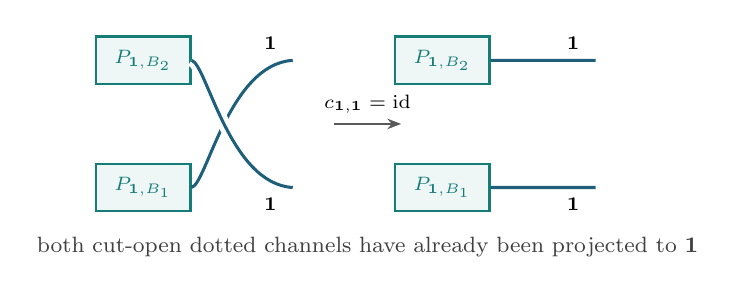
\begin{tikzpicture}[scale=.95]
  \node[projector coupon] (pl) at (-3,-.85) {$P_{\mathbf1,B_1}$};
  \node[projector coupon] (pr) at (-3,.85) {$P_{\mathbf1,B_2}$};
  \draw[plain strand] (pl.east) .. controls (-2.15,-.8) and (-1.85,.8) .. (-1,.85);
  \draw[plain strand,preaction={draw=white,line width=4.5pt}]
    (pr.east) .. controls (-2.15,.8) and (-1.85,-.8) .. (-1,-.85);
  \node[font=\scriptsize] at (-1.3,1.08) {$\mathbf1$};
  \node[font=\scriptsize] at (-1.3,-1.08) {$\mathbf1$};

  \draw[flow arrow] (-.45,0) -- (.45,0)
    node[midway,above,font=\scriptsize] {$c_{\mathbf1,\mathbf1}=\operatorname{id}$};

  \node[projector coupon] (ql) at (1,-.85) {$P_{\mathbf1,B_1}$};
  \node[projector coupon] (qr) at (1,.85) {$P_{\mathbf1,B_2}$};
  \draw[plain strand] (ql.east) -- (3.05,-.85);
  \draw[plain strand] (qr.east) -- (3.05,.85);
  \node[font=\scriptsize] at (2.75,1.08) {$\mathbf1$};
  \node[font=\scriptsize] at (2.75,-1.08) {$\mathbf1$};
  \node[semantic label] at (0,-1.65)
    {both cut-open dotted channels have already been projected to $\mathbf1$};
\end{tikzpicture}

  \caption{After simultaneous cutting, the $1/1$ calculation exchanges two
  tensor-unit channels.}
\end{figure}

\begin{figure}[ht]
  \centering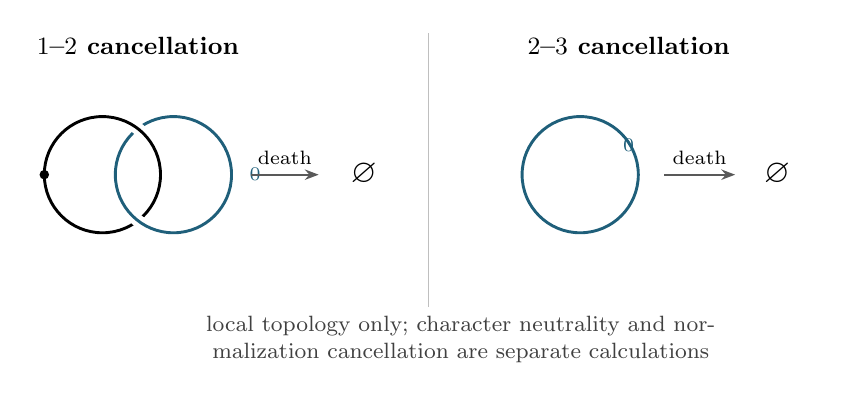
\begin{tikzpicture}[scale=.82]
  \node[font=\small\bfseries] at (-3.5,2) {$1$--$2$ cancellation};
  \begin{scope}[shift={(-3.5,0)}]
    \draw[kirby component] (-.55,0) circle[radius=.9];
    \draw[ordinary component,preaction={draw=white,line width=4.5pt}]
      (.55,0) circle[radius=.9];
    \draw[kirby component,preaction={draw=white,line width=4.5pt}]
      (-.55,0) ++(42:.9) arc[start angle=42,end angle=60,radius=.9];
    \fill (-1.45,0) circle[radius=2.1pt];
    \node[font=\scriptsize,text=TYordinary,anchor=west] at (1.58,0) {$0$};
  \end{scope}
  \draw[flow arrow] (-1.75,0) -- (-.7,0)
    node[midway,above,font=\scriptsize] {death};
  \node[font=\large] at (0,0) {$\varnothing$};

  \draw[black!25,line width=.6pt] (1,-2.05) -- (1,2.2);

  \node[font=\small\bfseries] at (4.1,2) {$2$--$3$ cancellation};
  \draw[ordinary component] (3.35,0) circle[radius=.9];
  \node[font=\scriptsize,text=TYordinary] at (4.1,.45) {$0$};
  \draw[flow arrow] (4.65,0) -- (5.75,0)
    node[midway,above,font=\scriptsize] {death};
  \node[font=\large] at (6.4,0) {$\varnothing$};
  \node[semantic label,text width=8.8cm] at (1.5,-2.55)
    {local topology only; character neutrality and normalization cancellation are separate calculations};
\end{tikzpicture}

  \caption{The local topology of the two cancellation moves.  Their scalar
  and normalization calculations are deliberately not hidden in the figure.}
\end{figure}

\end{document}
